\subsection{構築の管理}

構築は個人の作業に見えやすいが、実際には管理対象が多い。どのライフサイクルで進めるか、どの順で部品を作るか、いつ統合するか、何を測るか、どの依存関係を許すかによって、品質と進捗は大きく変わる。

\subsubsection{ライフサイクルモデルにおける構築}

ライフサイクルモデルによって、構築の位置づけは異なる。ウォーターフォール型や段階的提供型では、要求や設計がある程度完了した後に構築が始まる。この場合、構築は主にコーディングとデバッグとして見られやすい。

一方、進化的プロトタイピングやアジャイル開発では、要求、設計、構築、テストが重なり合う。短い反復の中で、必要な要求を具体化し、設計し、コードを書き、テストする。継続的デリバリや継続的デプロイでは、コード、テスト、提供、配置がさらに密接に結びつき、自動化されたパイプラインで実行される。

\par\smallskip
\begin{center}
\centering
\IfFileExists{assets/generated_figures/ch04/fig-ch04-04.png}{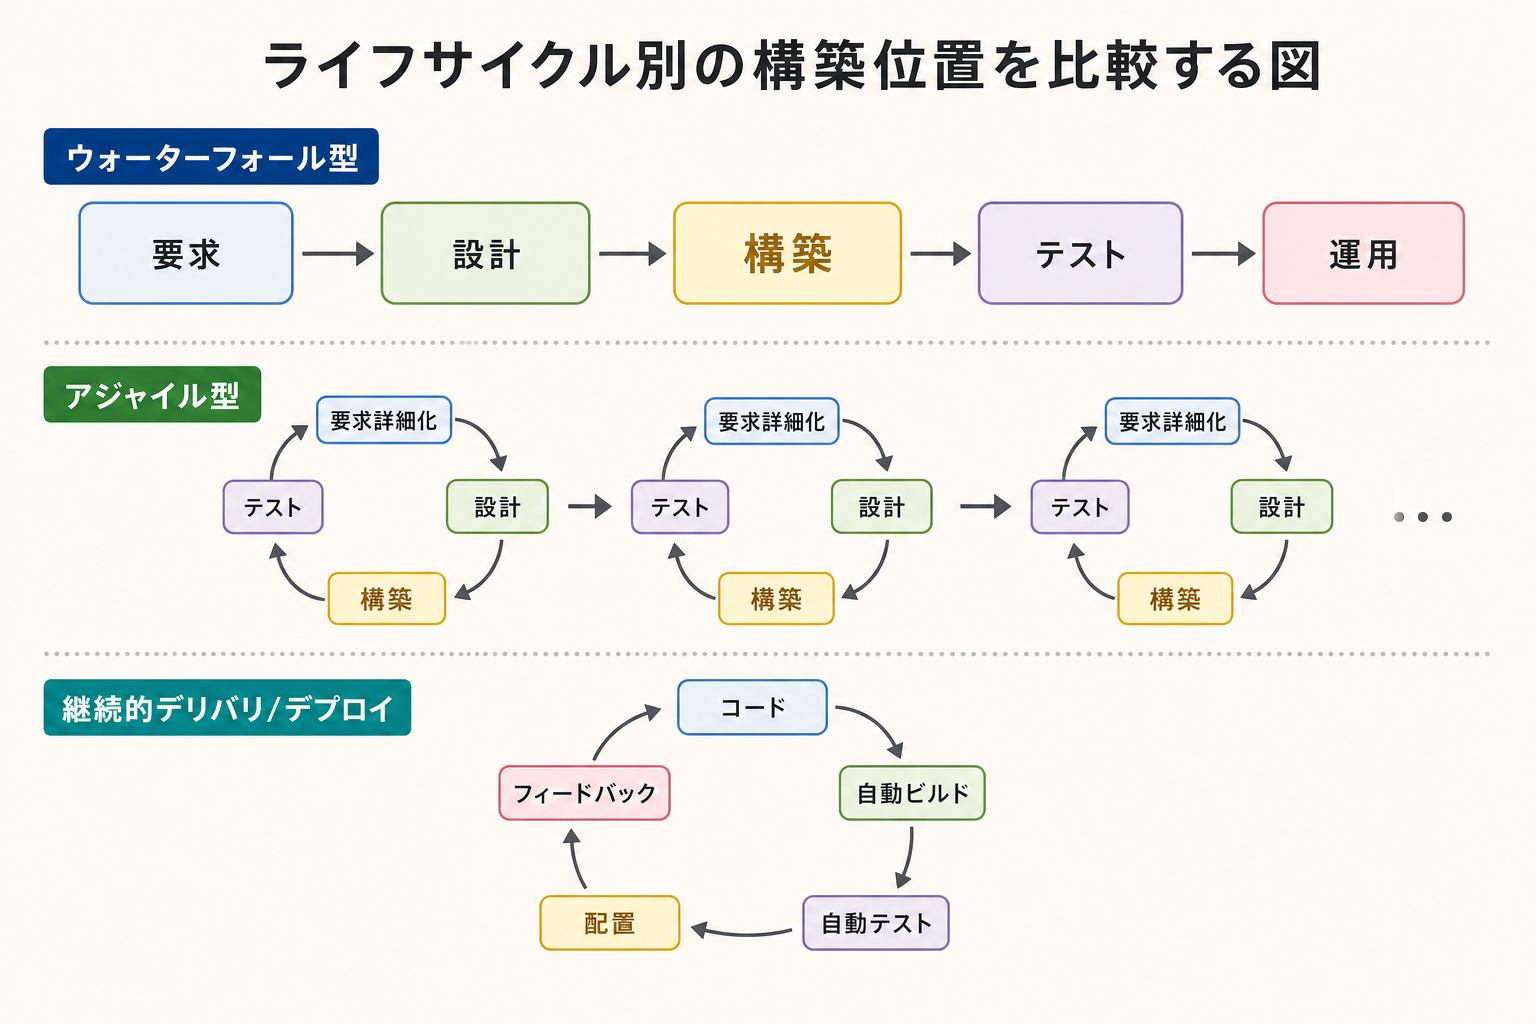
\includegraphics[width=0.96\linewidth]{assets/generated_figures/ch04/fig-ch04-04.png}}{\fbox{\parbox[c][48mm][c]{0.9\linewidth}{\centering 画像生成待ち\\ライフサイクル別の構築位置を比較する図}}}
\par\smallskip
\refstepcounter{figure}\label{fig:ch04-04}図 \thefigure: ライフサイクル別の構築位置を比較する図
\end{center}
図 \thefigure は、ライフサイクル別の構築位置を比較する図を視覚的に整理したものである。
\par\smallskip

\subsubsection{構築計画}

構築計画では、構築方法、部品の作成順序、統合順序、統合戦略、品質管理プロセス、担当割り当て、必要なツールや環境を決める。構築方法の選択は、複雑さの低減、変化への対応、検証しやすさに影響する。

たとえば、最初から全体を一度に統合する方針を選べば、初期の計画は単純に見えるが、問題発見が遅れる可能性がある。小さな部品を段階的に統合する方針を選べば、統合のための足場やテスト環境が必要になるが、問題を早く見つけやすい。

\subsubsection{構築測定}

構築では、多くの活動や成果物を測定できる。開発したコード量、変更したコード量、再利用したコード量、削除したコード量、コード複雑度、コードレビューで見つかった欠陥数、欠陥発見率、欠陥修正率、作業工数、予定との差分などである。

測定の目的は、管理と改善である。数値を集めるだけでは意味がない。たとえば、複雑度が高い箇所を重点的にレビューする、欠陥修正率から計画を見直す、再利用量から開発効率を評価する、といった使い方が必要である。

\subsubsection{依存関係の管理}

現代のソフトウェアは、多くの外部ライブラリやフレームワークに依存する。Java の Maven、JavaScript の NPM などのパッケージ管理ツールは、依存関係の導入、更新、削除を自動化する。しかし、依存関係は便利である一方、リスクも運ぶ。

依存関係の集合は、供給網のようなネットワークを作る。直接使っているライブラリが、さらに別のライブラリに依存していることも多い。どこかに脆弱性、ライセンス衝突、保守停止、悪意あるコードがあれば、自分の製品にも影響する。

依存関係管理では、不要な依存を避ける、信頼できる依存だけを使う、ライセンスを確認する、脆弱性情報を監視する、バージョン更新を計画する、ロックファイルやソフトウェア部品表を活用する、といった実践が重要である。

\par\smallskip
\begin{center}
\centering
\IfFileExists{assets/generated_figures/ch04/fig-ch04-05.png}{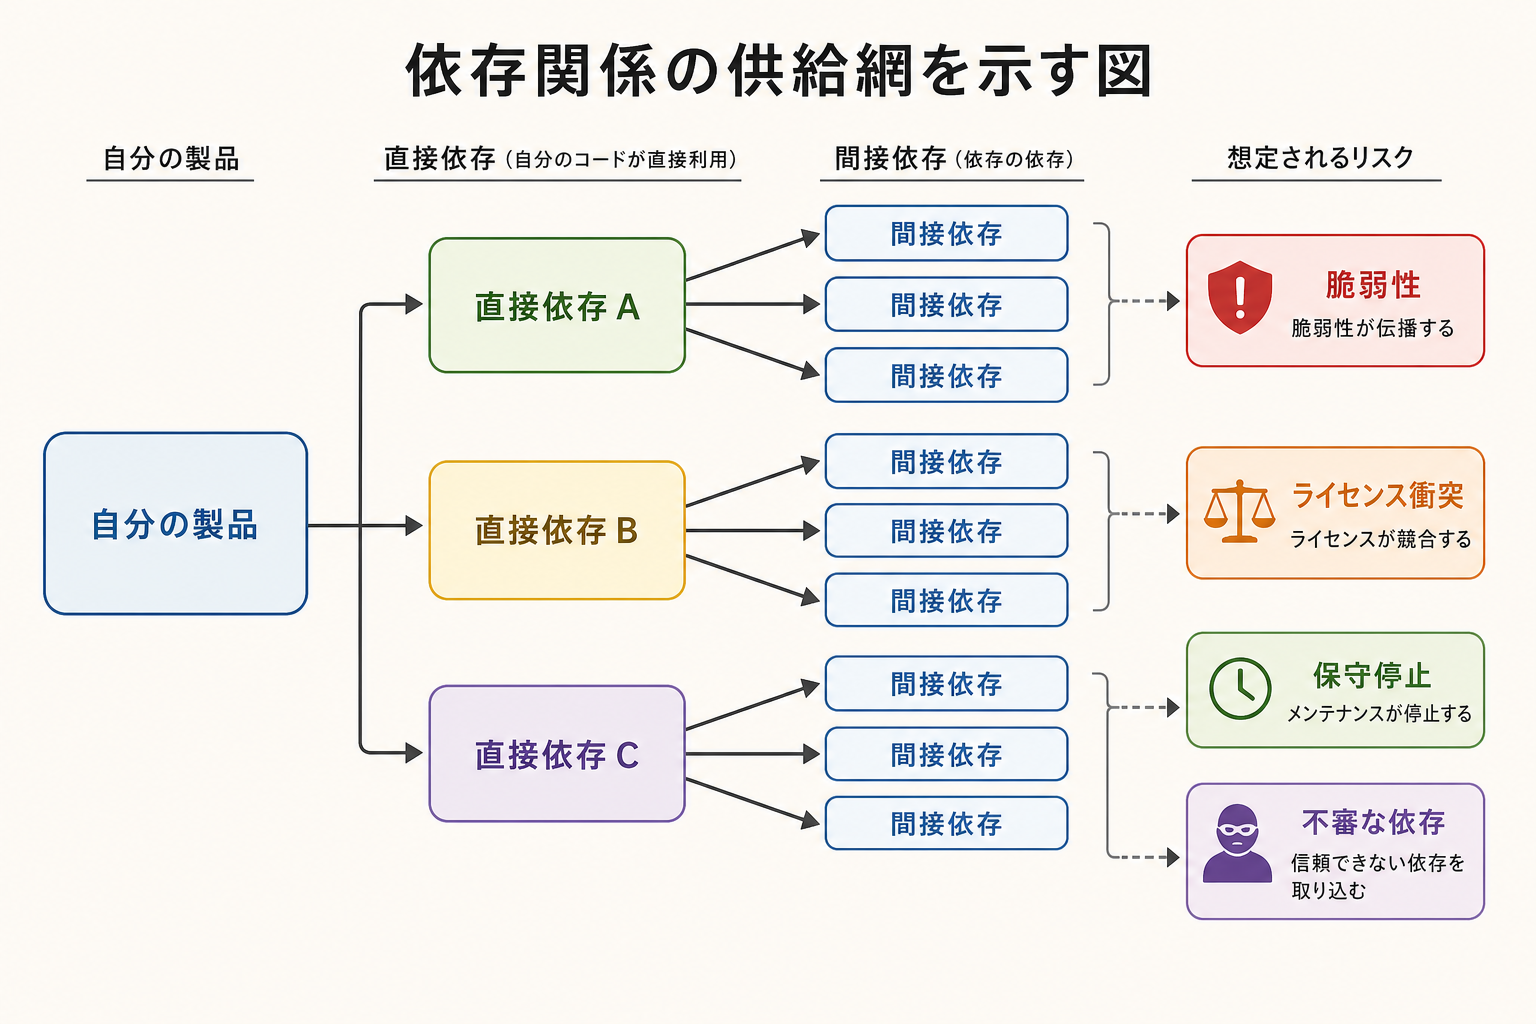
\includegraphics[width=0.96\linewidth]{assets/generated_figures/ch04/fig-ch04-05.png}}{\fbox{\parbox[c][48mm][c]{0.9\linewidth}{\centering 画像生成待ち\\依存関係の供給網を示す図}}}
\par\smallskip
\refstepcounter{figure}\label{fig:ch04-05}図 \thefigure: 依存関係の供給網を示す図
\end{center}
図 \thefigure は、依存関係の供給網を示す図を視覚的に整理したものである。
\par\smallskip
